\begin{tikzpicture}[yscale=6, xscale=3]
    \ShowGrid{(-2,0); (2,1)}
    % pdf
    \Plot[-2:2][teal]{1/(sqrt(0.2)*sqrt(2*pi))*exp(-(x-0)**2/(2*0.2**2))}
    \Plot[-2:2][orange]{1/(sqrt(0.5)*sqrt(2*pi))*exp(-(x-0)**2/(2*0.5**2))}
    \Plot[-2:2][green]{1/(sqrt(1)*sqrt(2*pi))*exp(-(x-0)**2/(2*1**2))}
    % cdf
    \Plot[-2:2][teal]{0.5*(1+erf((x-0)/(sqrt(0.2)*sqrt(2))))}
    \Plot[-2:2][orange]{0.5*(1+erf((x-0)/(sqrt(0.5)*sqrt(2))))}
    \Plot[-2:2][green]{0.5*(1+erf((x-0)/(sqrt(1)*sqrt(2))))}
    % annotate
    \ShowPoint[radius=0pt]{(-1, 0); (0, 0); (1, 0)}[$\mu-\sigma$; $\mu=0$; $\mu+\sigma$][below]
    \ShowPoint[radius=0pt]{(1, 0.8); (1, 0.6); (1, 0.4)}[
        \textcolor{red}{\rule[1pt]{8pt}{3pt}}\;$\sigma^2=0.2$;
        \textcolor{orange}{\rule[1pt]{8pt}{3pt}}\;$\sigma^2=0.5$;
        \textcolor{green}{\rule[1pt]{8pt}{3pt}}\;$\sigma^2=1$;
    ][right=2em]
    \ShowPoint[radius=0pt]{(-1, 0.8)}[$\displaystyle y = \frac{1}{\sigma\sqrt{2\pi}}\mathrm{Exp}\{-\frac{(x-\mu)^2}{2\sigma^2}\}$]
    \ShowPoint[radius=0pt]{(-1, 0.6)}[$y=\frac12\left(1+\mathrm{Erf}(\frac{x-\mu}{\sigma\sqrt{2}})\right)$]
\end{tikzpicture}